\newpage
\section{Theoretical Background}

\subsection{Linear Programming in Energy Systems}

At its core, our problem focuses on meeting electricity demand through optimal generation dispatch:
determining how much power each generator should produce to satisfy consumer demand while minimizing costs 
and respecting system constraints. This fundamental power systems challenge can be effectively modeled using 
Linear Programming (LP).
\begin{figure}[h]
    \centering
    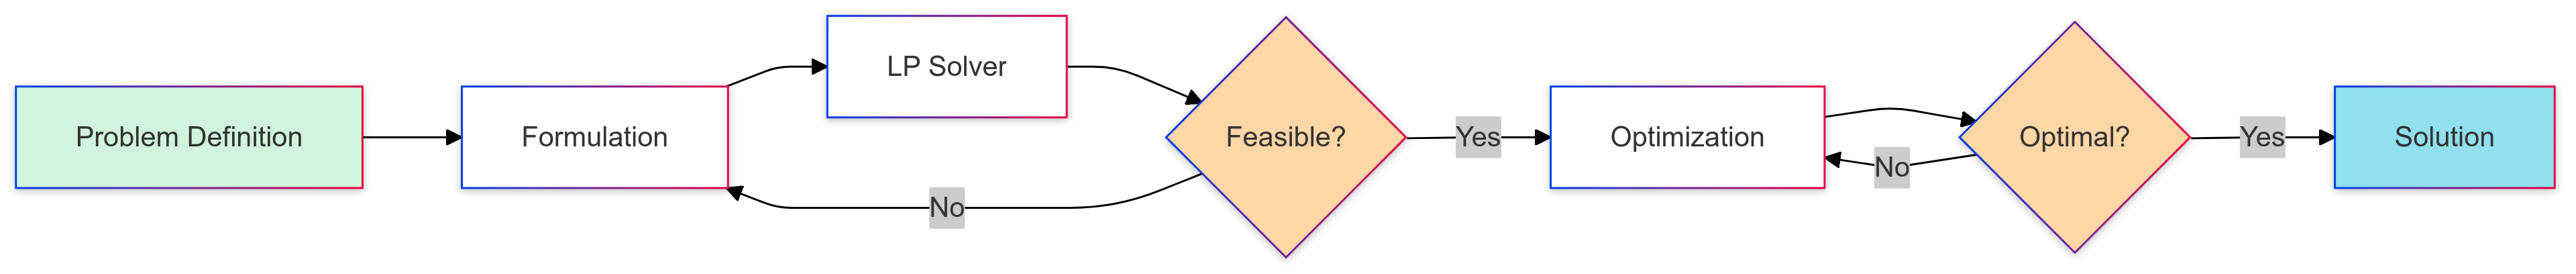
\includegraphics[width=0.8\textwidth]{images/lp_flowchart.png}
    \caption{LP optimization flowchart showing key steps from problem formulation to optimal solution.} \label{fig:lp_flowchart}
\end{figure}

Linear Programming enables modeling of key power system relationships - such as power balance(matching
generation to demand), transmission limits, and generation constraints - as linear equations and inequalities. 
The basic structure of our optimization problem is:

\begin{itemize}
    \item \textbf{Objective}: Minimize total generation cost
    \item \textbf{Primary Decision}: How much power to generate at each plant
    \item \textbf{Key Constraint}: Total generation must meet demand at all times
    \item \textbf{System Constraints}: Respect network and equipment limitations
\end{itemize}

This can be expressed mathematically as:

\begin{equation}
    \min_{\mathbf{x}} \mathbf{c}^\top \mathbf{x} \quad \text{subject to} \quad A\mathbf{x} \leq \mathbf{b}
\end{equation}

\subsection{DC Optimal Power Flow}
The DC Optimal Power Flow (DC-OPF) extends the basic generation dispatch problem by incorporating network constraints.
It answers the question: "How should we distribute power generation across the network to meet demand
at minimum cost while respecting transmission line limits?" The DC-OPF achieves this by:
\begin{itemize}
    \item Modeling power flow through transmission lines
    \item Ensuring power balance at each network node
    \item Respecting both generation and transmission limits
\end{itemize}

The "DC" prefix indicates a linearized approximation of the full AC power flow equations, making the problem
 solvable using LP techniques~\cite{wood2013power}. This approximation is particularly effective for 
 high-voltage transmission planning~\cite{andersson2004power}.

\subsubsection{Key Assumptions}
The DC approximation makes four key simplifications:
\begin{itemize}
    \item Voltage magnitudes are fixed at 1.0 per unit
    \item Line resistances are negligible ($R \ll X$)
    \item Voltage angle differences are small
    \item Reactive power (power that oscillates between source and load without doing useful work) is ignored
\end{itemize}

These assumptions yield a simple relationship between power flow ($P_{ij}$) and voltage angles ($\theta$):
\begin{equation}
    P_{ij} = B_{ij}(\theta_i - \theta_j)
\end{equation}

\subsubsection{Mathematical Formulation}
The DC-OPF problem minimizes generation costs subject to network constraints. Each equation represents a 
physical aspect of power system operation:

\vspace{0.5cm}
\textbf{1. Power Balance} - The fundamental law of power systems
\begin{itemize}
    \item At each bus $i$, power in equals power out
    \item Generation minus demand equals net power flow to neighboring buses
    \item Determined by line susceptances and voltage angles
\end{itemize}
\begin{equation}
    \sum_{g \in \mathcal{G}_i} P_{g,t} - D_{i,t} = \sum_{j \in \mathcal{N}_i} B_{ij}(\theta_{i,t} - \theta_{j,t}) \quad \forall i \in \mathcal{N}, t \in \mathcal{T}
\end{equation}

\vspace{0.5cm}
\textbf{2. Cost Minimization} - Economic objective
\begin{itemize}
    \item Find optimal generation dispatch that minimizes total system cost
    \item Each generator has an associated marginal cost function (cost per unit of production)
\end{itemize}
\begin{equation}
    \min_{\mathbf{P_g}, \boldsymbol{\theta}} \sum_{g \in \mathcal{G}} \sum_{t \in \mathcal{T}} c_g P_{g,t}
\end{equation}

\vspace{0.5cm}
\textbf{3. Line Capacity} - Network limitations
\begin{itemize}
    \item Power flow must stay within thermal limits of transmission lines
    \item Bi-directional constraint (forward and reverse flow limits)
\end{itemize}
\begin{equation}
    -P_{ij}^{\max} \leq B_{ij}(\theta_{i,t} - \theta_{j,t}) \leq P_{ij}^{\max} \quad \forall (i,j) \in \mathcal{L}, t \in \mathcal{T}
\end{equation}

\vspace{0.5cm}
\textbf{4. Generator Limits} - Physical constraints
\begin{itemize}
    \item Each generator is limited by minimum and maximum output
    \item Generators may have time-varying limits
\end{itemize}
\begin{equation}
    P_{g}^{\min} \leq P_{g,t} \leq P_{g}^{\max} \quad \forall g \in \mathcal{G}, t \in \mathcal{T}
\end{equation}

\vspace{0.5cm}
\textbf{5. Reference Angle} - System reference
\begin{itemize}
    \item One bus sets the reference for voltage angles
    \item Typically chosen as the largest generator
\end{itemize}
\begin{equation}
    \theta_{\text{slack},t} = 0 \quad \forall t \in \mathcal{T}
\end{equation}

\subsubsection{Storage System Constraints}
The model includes battery storage systems with the following constraints:

\vspace{0.5cm}
\textbf{1. Energy Balance} - Storage state evolution
\begin{itemize}
    \item Tracks energy level over time
    \item Accounts for charging and discharging efficiencies
\end{itemize}
\begin{equation}
    E_{s,t+1} = E_{s,t} + \eta_c P_{c,s,t} - \frac{P_{d,s,t}}{\eta_d} \quad \forall s \in \mathcal{S}, t \in \mathcal{T}
\end{equation}

\vspace{0.5cm}
\textbf{2. Power Limits} - Operational boundaries
\begin{itemize}
    \item Maximum charging and discharging rates
    \item Cannot charge and discharge simultaneously
\end{itemize}
\begin{equation}
    0 \leq P_{c,s,t} \leq P_{c,s}^{\max} \quad \forall s \in \mathcal{S}, t \in \mathcal{T}
\end{equation}
\begin{equation}
    0 \leq P_{d,s,t} \leq P_{d,s}^{\max} \quad \forall s \in \mathcal{S}, t \in \mathcal{T}
\end{equation}

\vspace{0.5cm}
\textbf{3. Energy Capacity} - Storage limits
\begin{itemize}
    \item Maximum and minimum state of charge
    \item Often includes end-state condition
\end{itemize}
\begin{equation}
    E_{s}^{\min} \leq E_{s,t} \leq E_{s}^{\max} \quad \forall s \in \mathcal{S}, t \in \mathcal{T}
\end{equation}
\begin{equation}
    E_{s,T} = E_{s,0} \quad \forall s \in \mathcal{S}
\end{equation}

Where:
\begin{itemize}
    \item $E_{s,t}$: Energy stored in battery $s$ at time $t$
    \item $P_{c,s,t}, P_{d,s,t}$: Charging and discharging power
    \item $\eta_c, \eta_d$: Charging and discharging efficiencies
\end{itemize}

\subsubsection{Implementation Considerations}
The model is implemented in Python using PuLP~\cite{mitchell2011pulp}, an open-source optimization framework, 
with the COIN-OR Branch and Cut (CBC) solver~\cite{forrest2018cbc}. As a first programming project, the 
focus was on developing a functional and flexible platform rather than computational optimization. This 
approach prioritized code clarity and feature implementation over algorithmic efficiency.

Howevere, our implementation processes hourly data for generator availability and demand profiles. For a full
 year analysis, this represents over 8,700 objective functions, each generating multiple constraints per time
  period. Real power systems often require even finer temporal resolution (15-minute intervals), more 
  elaborate constraints. This is a simplified model but grasps the core principles of the problem.

To manage computational complexity, we use representative weeks selection for seasonal patterns. Involves 
some uncertainty, but allows meaningful analysis while improving computing time by a factor 20-30x. Future 
work could focus on algorithmic improvements and computational optimization.
